\documentclass[a4paper]{article}

% Global layout
\usepackage{fancyhdr, graphicx, hyperref, indentfirst, lastpage, setspace}
\usepackage{geometry}

% Encoding
\usepackage[utf8]{vntex, inputenc}
\usepackage[english]{babel}
\usepackage{amsmath, amssymb, gensymb}

% Better table
\usepackage{array, booktabs, multicol, multirow, siunitx, tabularx}

% Code space
\usepackage[dvipsnames]{xcolor}
\usepackage{tikz}
\usepackage[framemethod=tikz]{mdframed}
\usepackage{minted, verbatim} % needs --shell-escape flag and Pygments

% Graphics
\usepackage{caption, float}

% Bullets & numbering
\usepackage{enumitem}

% Page setup
\allowdisplaybreaks{} % to have page breaks inside align* environment
\hypersetup{urlcolor=blue,linkcolor=black,citecolor=red,colorlinks=true}
\usemintedstyle{emacs}
\numberwithin{equation}{section}
\renewcommand{\arraystretch}{1.2} % space between table rows

% Global style setup
\makeatletter % change font size for not having underfull hbox
\renewcommand\Huge{\@setfontsize\Huge{22pt}{18}}
\makeatother

\AtBeginDocument{\renewcommand*\contentsname{Contents}}
\AtBeginDocument{\renewcommand*\refname{References}}
\setlength{\headheight}{40pt}
\pagestyle{fancy}
\fancyhead{} % clear all header fields
\fancyhead[L]{
  \begin{tabular}{rl}
    \begin{picture}(25,15)(0,0)
    \put(0,-8){
\includegraphics[width=8mm, height=8mm]{./assets/hcmut.png}}
    \end{picture}
    \begin{tabular}{l}
      \textbf{\bf \ttfamily University of Technology, Ho Chi Minh City}\\
      \textbf{\bf \ttfamily Faculty of Computer Science and Engineering}
    \end{tabular}
  \end{tabular}
}
\fancyhead[R]{
	\begin{tabular}{l}
		\tiny \bf \\
		\tiny \bf
	\end{tabular}  }
\fancyfoot{} % clear all footer fields
\fancyfoot[L]{\scriptsize \ttfamily Programming Integration Project --- Academic year 2021--2022}
\fancyfoot[R]{\scriptsize \ttfamily Page {\thepage}/\pageref{LastPage}}
\renewcommand{\headrulewidth}{0.3pt}
\renewcommand{\footrulewidth}{0.3pt}

% \everymath{\color{blue}}

\newcommand*\mean[1]{\bar{#1}}
\newenvironment{code}[1]
{\VerbatimEnvironment%
  \begin{mdframed}[leftline=false,rightline=false,backgroundcolor=magenta!10,nobreak=false]%
    \begin{minted}[linenos=true,breaklines,breaksymbolleft=,obeytabs=true,tabsize=2]{#1}%
}
{
    \end{minted}%
  \end{mdframed}%
}

\begin{document}

\begin{titlepage}
  \begin{center}
    VIETNAM NATIONAL UNIVERSITY, HO CHI MINH CITY \\
    UNIVERSITY OF TECHNOLOGY \\
    FACULTY OF COMPUTER SCIENCE AND ENGINEERING
  \end{center}

  \vspace{1cm}

  \begin{figure}[H]
    \centering
    
\includegraphics[width=0.5\textwidth]{./assets/hcmut.png}
  \end{figure}

  \vspace{1cm}

  \begin{center}
    \begin{tabular}{c}
      \textbf{\Large Programming Integration Project (CO3103)} \\
      {}                                                       \\
      \midrule                                                 \\
      \textbf{\Large Project Report}                           \\
      {}                                                       \\
      \textbf{\Huge Mobile Phone Selling Website}              \\
      {}                                                       \\
      \bottomrule
    \end{tabular}
  \end{center}

  \vspace{3cm}

  \begin{table}[h]
    \begin{tabular}{rl}
      \hspace{1cm} Advisor: & Prof.\ Quản Thành Thơ \\
    \end{tabular}
  \end{table}

  \begin{center}
    {\footnotesize HO CHI MINH CITY, OCTOBER 2021}
  \end{center}
\end{titlepage}

\tableofcontents
\newpage

%\thispagestyle{empty}
\section*{Member list}
\begin{center}
  \begin{tabular}{llc}
    \toprule
    \textbf{No.} & \textbf{Full name} & \textbf{Student ID} \\
    \midrule
    1            & Nguyễn Hoàng       & 1952255             \\
    2            & Nguyễn Chính Khôi  & 1952793             \\
    3            & Vũ Anh Nhi         & 1952380             \\
    4            & Lương Duy Hưng     & 1952747             \\
    \bottomrule
  \end{tabular}
\end{center}

\newpage

\section{Topic}
This project focuses on creating a web-based application that allows users or customers to browse and make transactions.
The specific target of product is phone, primarily smart mobile device.

This e-commerce application is analogous to real life phone selling retailers that require a more convenient and efficient way for customers to interact with their products.
Because of that, the requirements and features will mainly focus on practical demands as if it was proposed to solve the problem.

\subsection{Proposed Features}
\begin{center}
  \begin{tabular}{*{2}{l}}
    \toprule
    Name                                     & Descriptions                                      \\
    \midrule
    Get news \& offers                       & Display current news and offers                   \\
    View catalog                             & Display list of products                          \\
    Place orders                             & Add items to cart                                 \\
    Authenticate Member account              & Login with username and password, (optional: SSO) \\
    Store member account's balance \& points & Save  purchases to calculate points               \\
    Create coupons                           & Validate coupons when checking out                \\
    Display statistics                       & Generate monthly sales of reports (Optional)      \\
    \bottomrule
  \end{tabular}
\end{center}

\subsection{Proposed workload}
\begin{center}
  \begin{tabular}{*{3}{l}}
    \toprule
    Task                                  &          & Member        \\
    \midrule
    Create database \& connect to backend &          & Hoàng \& Hưng \\
    Create mock-up homepage               &          & Nhi \& Khôi   \\
    Account registration and login        & Frontend & Khôi          \\
                                          & Backend  & Hưng          \\
    News and catalogue                    & Frontend & Nhi           \\
                                          & Backend  & Hưng          \\
    \bottomrule
  \end{tabular}
\end{center}

\section{Tools \& Technologies}

% Advantages/ Disadvantages
% Reasons why we choose this
% Basic features

We decided to make the backend serve a RESTful API, so that we can decouple the server and client as well as ensuring ease of scale should that ever happen.
With that said, we chose to demonstrate this project as a web application.

\begin{enumerate}[label=\alph*.]

  \item Frontend: \textbf{React}

        React (React.js or ReactJS) is a free and open-source front-end JavaScript library for building user interfaces or UI components.
        Developed at Facebook and released in 2013, it can be said that React has been the most influential UI library of recent years.

        We use React to build components that represent logical reusable parts of the UI\@.
        The beauty of React is that the simplicity of building a component has been brought down to its theoretical minimum: a Javascript function.
        The return value from these functions is the HTML or UI, which is written in a special syntax called JSX, allowing easy combination of Javascript with Html markup.

        The main reason we want to use React is not the library itself but the massive ecosystem surrounding it.
        React itself does not care about routing state management, animation or anything like that.
        Instead, it lets those concerns evolve naturally within the open-source community.
        No matter what we are trying to do, there is a good chance that a good supporting library to help us get it done has already existed.

  \item Backend: \textbf{NestJS}

        NestJS is a Node.js framework for building scalable server-side applications with Typescript.
        It comes with a ton of built-in modules to work with databases, handle security, implement streaming and anything else you can imagine doing in a server-side application.

        Using the NestJS CLI, you can scaffold out a new project with a code base pre-configured with Jest for testing and set up with Typescript to write more readable and reliable code.

  \item Database: \textbf{PostgreSQL}

        PostgreSQL is a powerful, open source object-relational database system that uses and extends the SQL language combined with many features that safely store and scale the most complicated data workloads.

        With more than 30 years of active development on the core platform, PostgreSQL has earned a strong reputation for its proven architecture, reliability, data integrity and more.
\end{enumerate}

\section{Mock-ups}

We have sketched the design of four pages that is in the scope of this project.
They are the \texttt{Home} page, \texttt{Product} (displaying list of products) page, \texttt{Product Detail}, and \texttt{View Cart} page.
We also sketched the \texttt{log in} pop-up window if customers clicked on the icon.
%, and the \texttt{show cart} pop-up window if you hover the mouse to the cart icon on the navigation bar.

This is the general flow of the website.
Most of the pages are linked by the buttons on the navigation bar.

\begin{figure}[H]
  \centering
  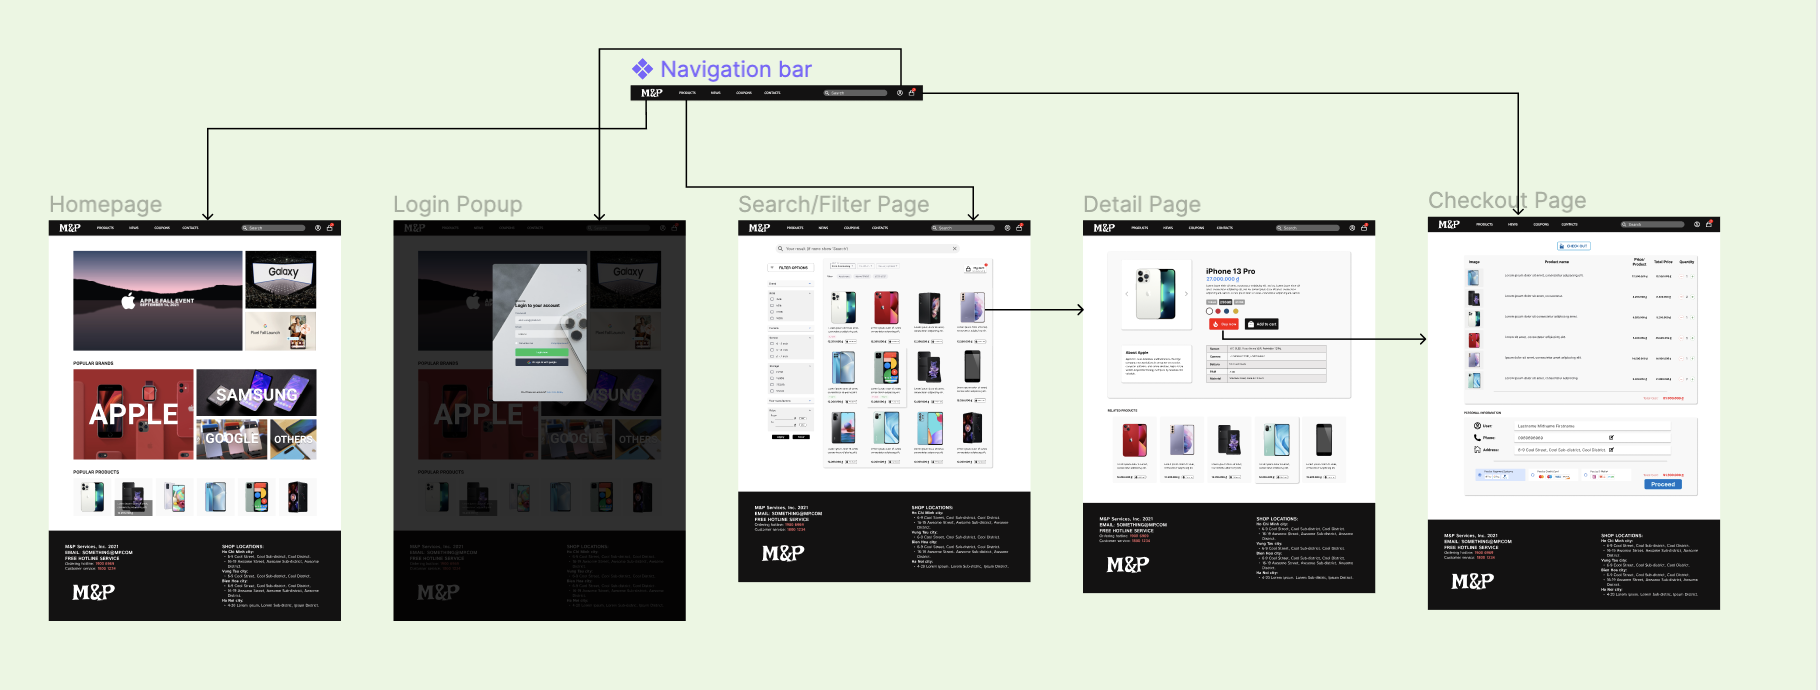
\includegraphics[width=0.8\textwidth]{assets/p2/screenflow.png}
  \caption{General Screen Flow}
\end{figure}

\begin{figure}
  \centering
  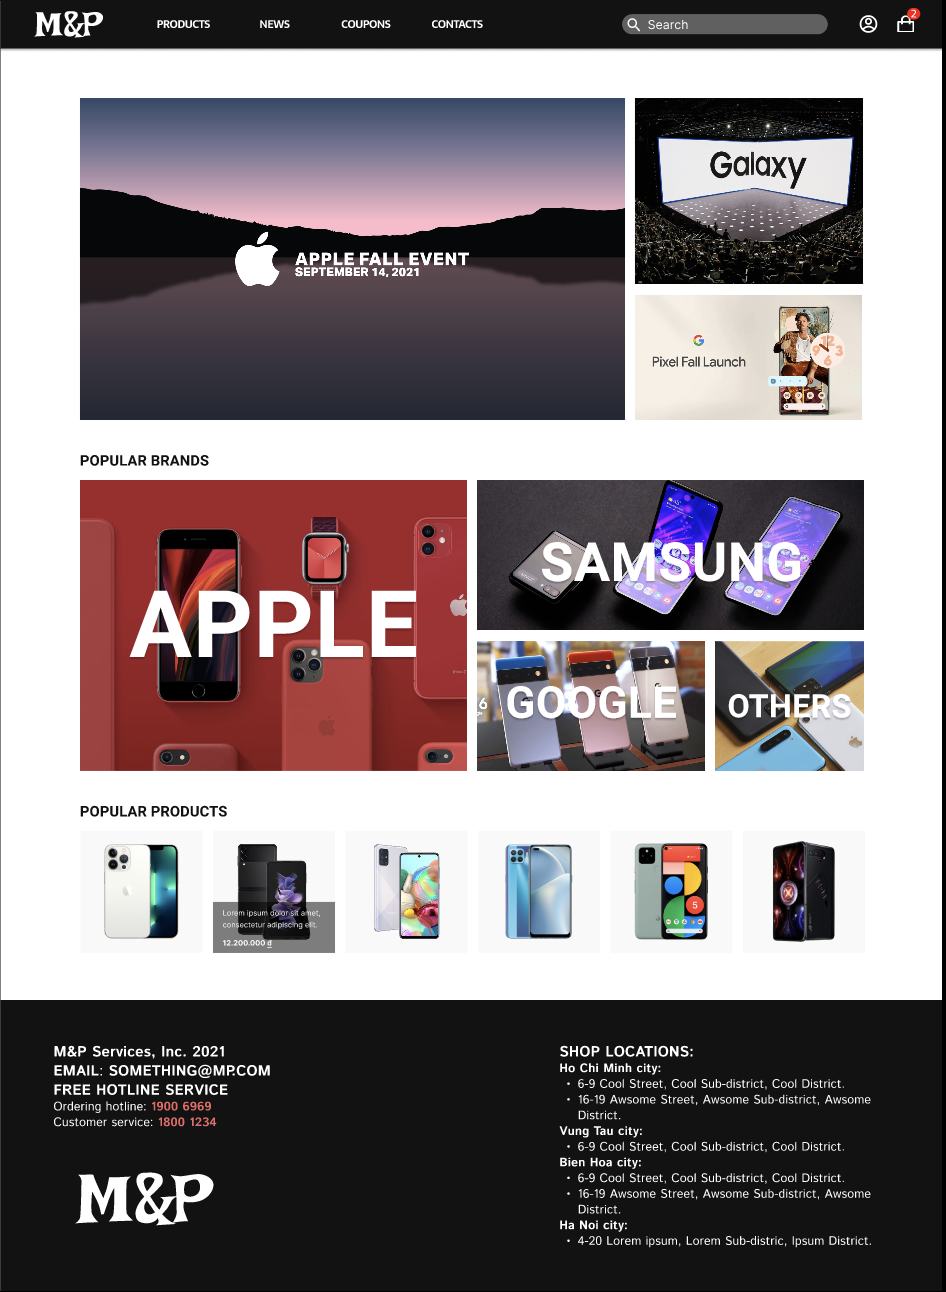
\includegraphics[width=0.8\textwidth]{assets/p2/p1.png}
  \caption{Homepage}
\end{figure}

These are the screenshots of the pages we designed using \texttt{Figma}.
\texttt{Figma} is a vector graphics editor and prototyping tool, which is suitable for basic UI design.
For a higher resolution view, please see the link \href{https://www.figma.com/proto/VaFUVfikhd1N98XmaqhA4p/Mock-up?node-id=35\%3A2504&scaling=scale-down-width&page-id=0\%3A1}{Mock-up}.

\begin{figure}
  \centering
  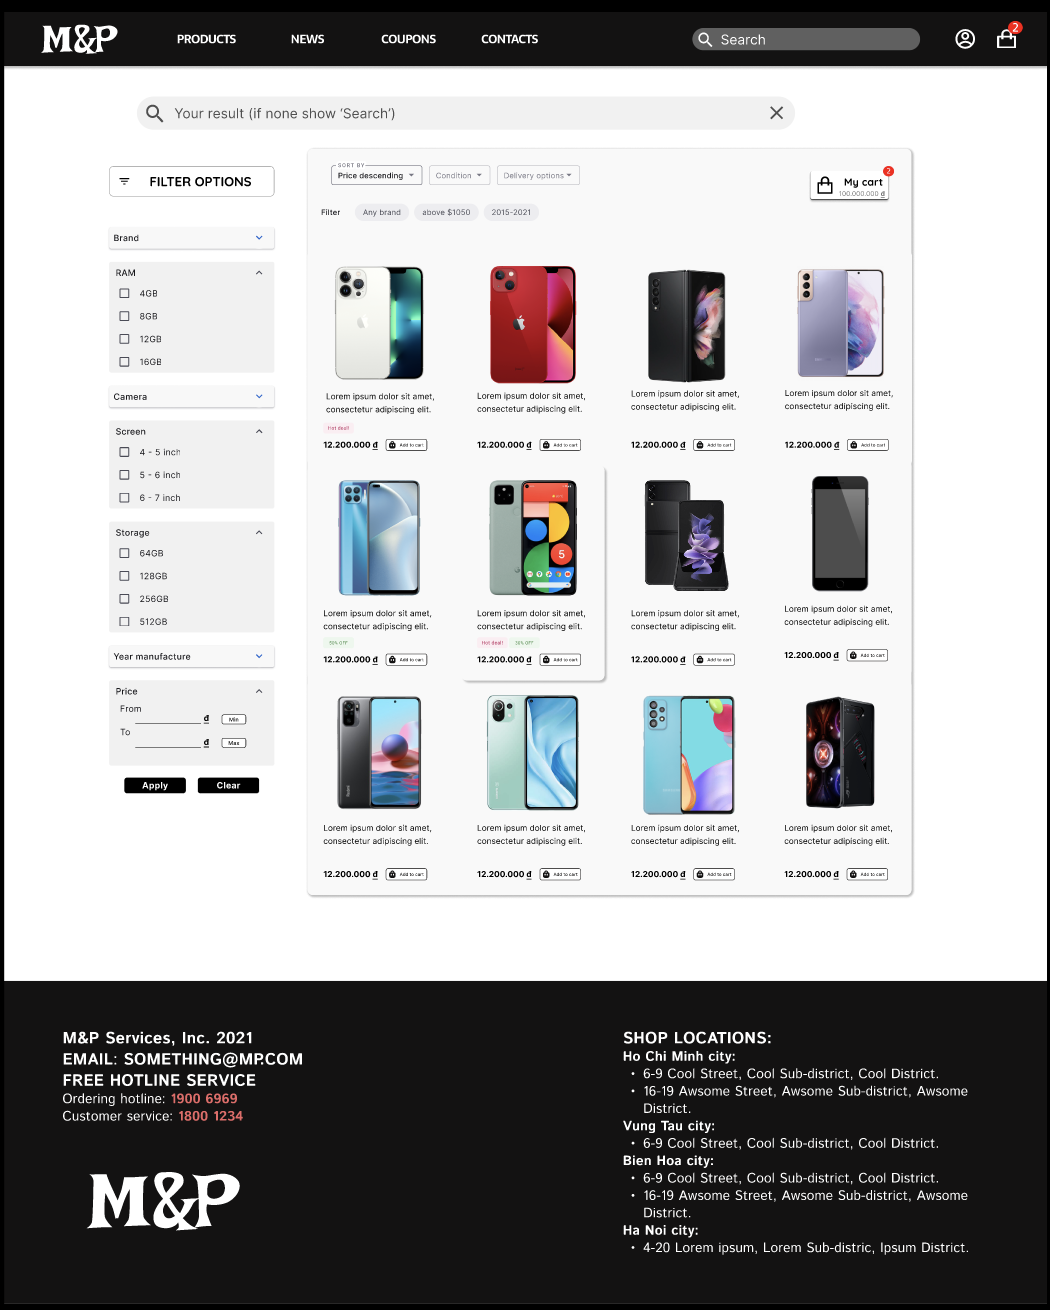
\includegraphics[width=0.9\textwidth]{assets/p2/p2.png}
  \caption{List of Products}
\end{figure}

\begin{figure}
  \centering
  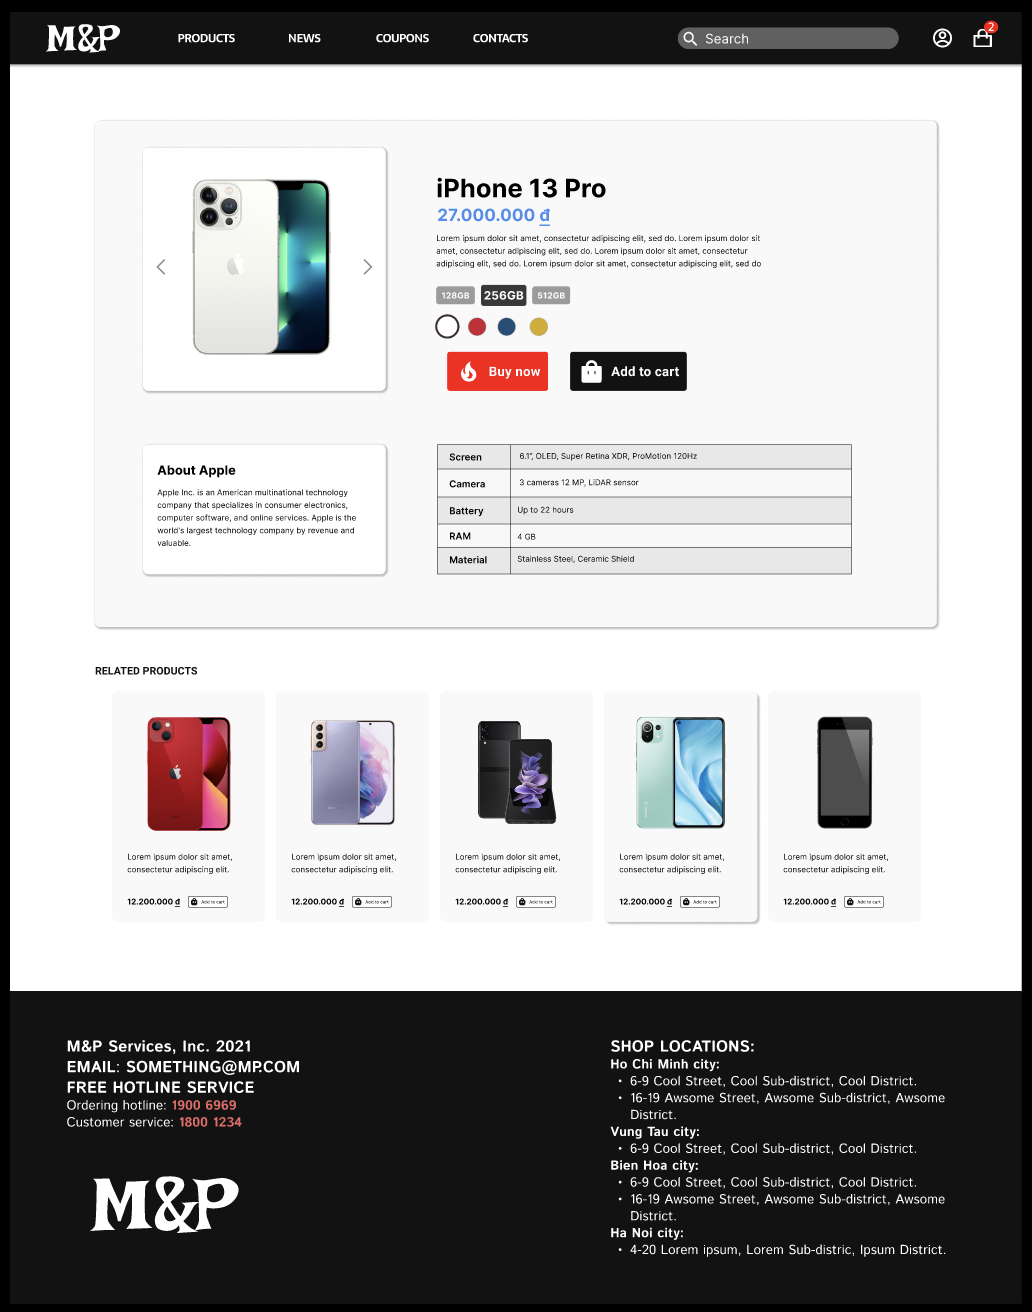
\includegraphics[width=0.9\textwidth]{assets/p2/p3.png}
  \caption{Product Details}
\end{figure}

\begin{figure}
  \centering
  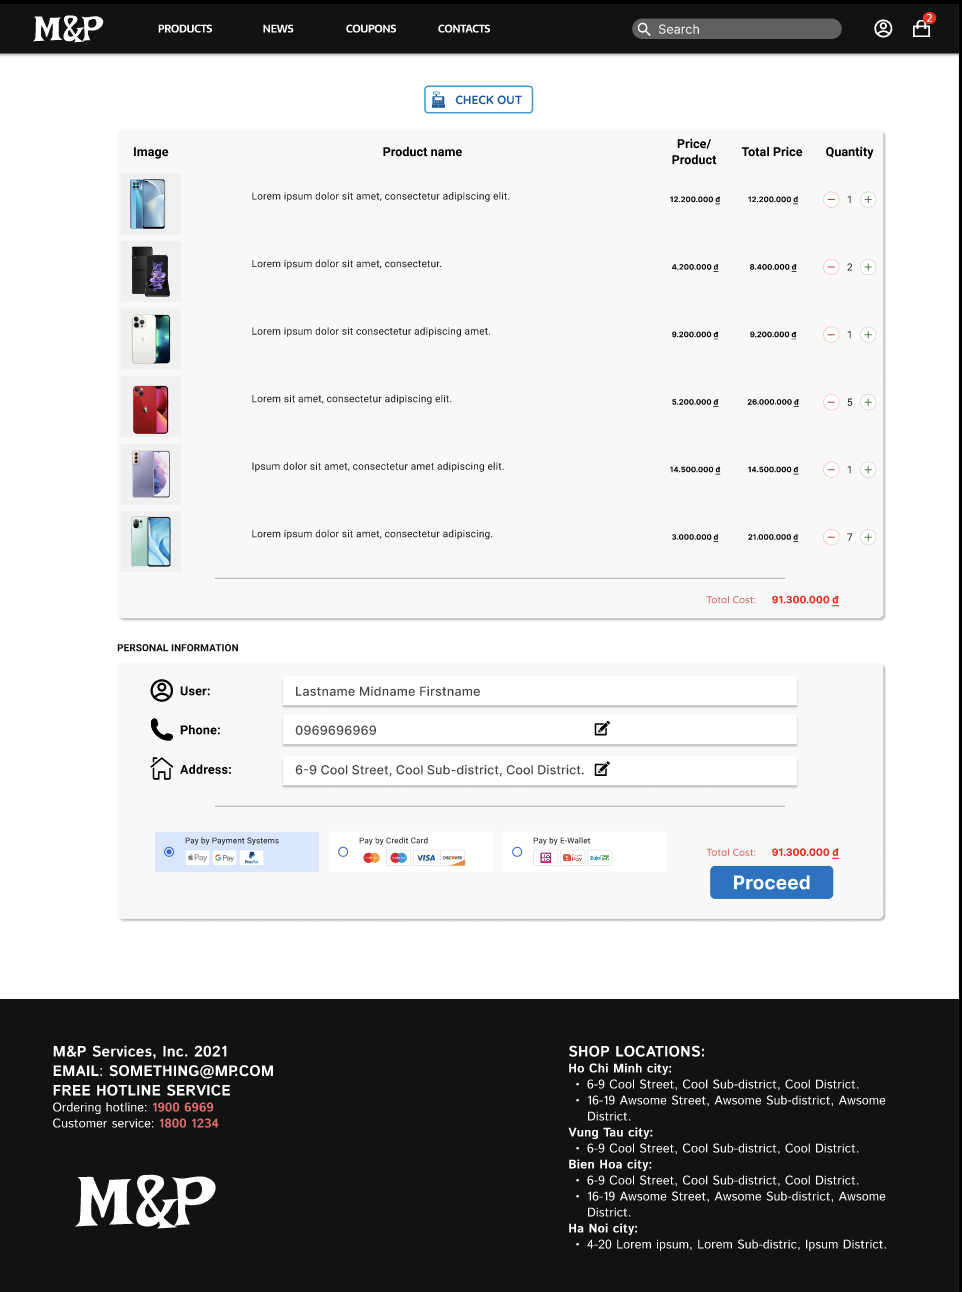
\includegraphics[width=0.9\textwidth]{assets/p2/p4.png}
  \caption{View Cart}
\end{figure}

\newpage
\section{Technologies \& Features}
So far, we have been learning about the thinking process of a developer.
For this integration project, we decided to practice this thinking process using some new frameworks.
At this point, we have already picked our tools, and after hours of research, we draw the conclusion on how all these technologies work and work together.

\subsection{Frontend}
\subsubsection{Component Reuse}
Why would you constantly reinvent the wheel when you can simply reuse code that has already been written and tested by other developers?

ReactJS introduces the so-called components, which make it possible to split the UI into independent, reusable pieces, and think about each piece in isolation.

For instance, we can have a button component display with different colors in several parts of our application.
Although it is the same button component when we provide it with a data set (e.g color, or a function), it modifies itself and outputs a UI instance of the element.

This pattern of creating React components is necessary for scaling.
It helps save time by ensuring less code is written, development is faster, the code base is simpler, and maintenance is stress-free.

\subsubsection{Virtual DOM}
The Document Object Model (DOM) is an application programming interface that represents an XML document as a tree structure wherein each node is an object representing a part of the document.

Most often it’s inefficient and slow because it’s necessary to recalculate the CSS, recreate the layout, and essentially repaint the entire web page every time the DOM changes.

ReactJS overcomes the DOM’s inefficiencies by using the so-called Virtual DOM\@.

Just like the actual DOM, the Virtual DOM represents all elements and their attributes as a node tree.
When something changes, React JS updates the Virtual DOM and figures out how it differs from the actual DOM, updating the actual DOM only with what has actually changed.

\subsubsection{JSX}
ReactJS introduces another concept called JSX, and it is a syntax extension to JavaScript.

React embraces the fact that rendering logic is inherently coupled with other UI logic: how events are handled, how the state changes over time, and how the data is prepared for display.

Instead of artificially separating technologies by putting markup and logic in separate files, React separates concerns with loosely coupled units called “components” that contain both.

React doesn’t require using JSX, but most people find it helpful as a visual aid when working with UI inside the JavaScript code. It also allows React to show more useful error and warning messages.

\subsection{Backend}
\begin{figure}[H]
  \centering
  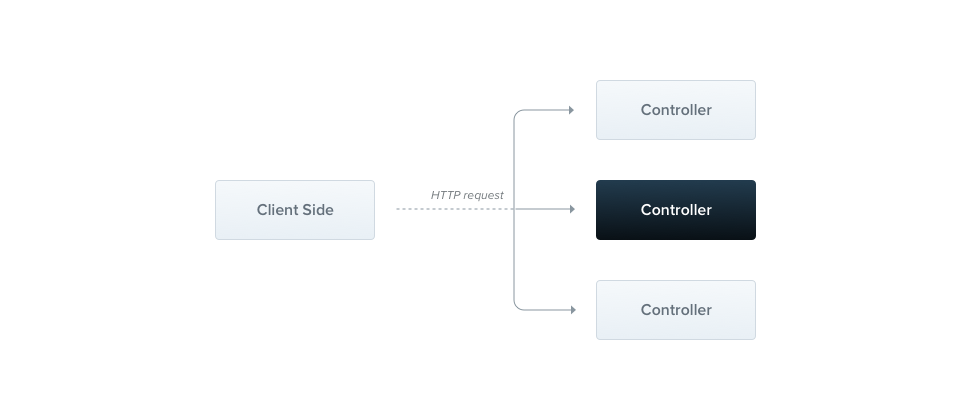
\includegraphics[width=0.8\textwidth]{./assets/p2/Controllers_1.png}
\end{figure}

\subsubsection{Controllers}
A controller's purpose is to receive specific requests for the application.
The routing mechanism controls which controller receives which requests.
Frequently, each controller has more than one route, and different routes can perform different actions.

\subsubsection{Providers}
\begin{figure}[H]
  \centering
  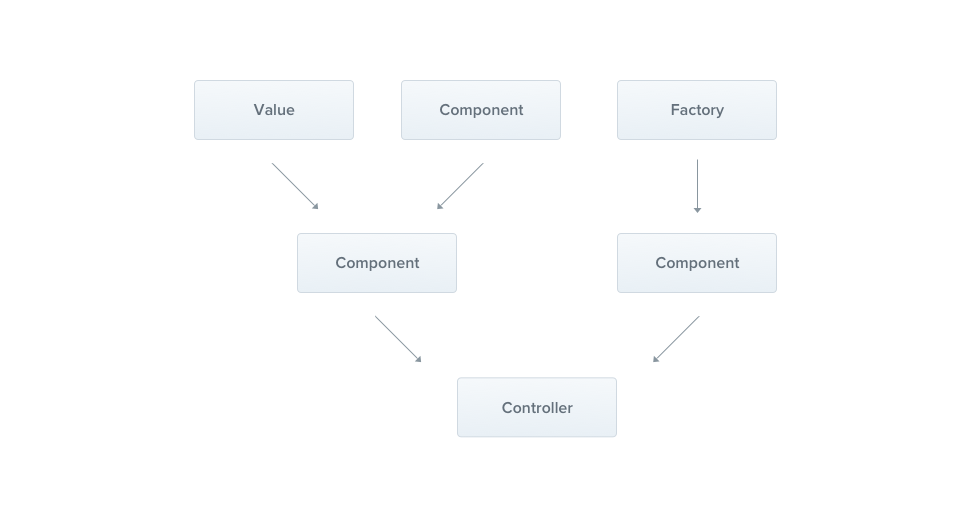
\includegraphics[width=0.8\textwidth]{./assets/p2/Providers_1.png}
\end{figure}

Nest introduces a new concept called providers.
Many of the basic Nest classes may be treated as a provider --- services, repositories, factories, helpers, and so on.
The main idea of a provider is that it can be injected as dependency; this means objects can create various relationships with each other, and the function of ``wiring up'' instances of objects can largely be delegated to the Nest runtime system.

\subsubsection{Modules}
\begin{figure}[H]
  \centering
  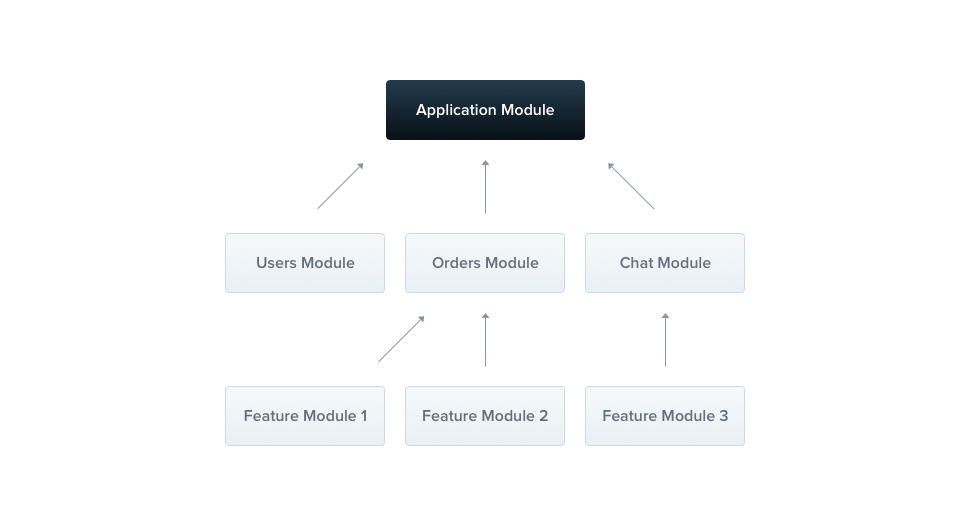
\includegraphics[width=0.8\textwidth]{./assets/p2/Modules_1.png}
\end{figure}

Each application has at least one module, a root module.
The root module is the starting point Nest uses to build the application graph --- the internal data structure Nest uses to resolve module and provider relationships and dependencies.

While very small applications may theoretically have just the root module, this is not the typical case.
We want to emphasize that modules are strongly recommended as an effective way to organize your components.
Thus, for most applications, the resulting architecture will employ multiple modules, each encapsulating a closely related set of capabilities.

The module encapsulates providers by default. This means that it's impossible to inject providers that are neither directly part of the current module nor exported from the imported modules. Thus, you may consider the exported providers from a module as the module's public interface, or API\@.

\end{document}
